\documentclass[9pt]{beamer}

\usepackage[T1]{fontenc}
\usepackage{color}
\usepackage{graphicx}
\usepackage{natbib}
\usepackage{tikz}
\usepackage{xmpmulti}
\usepackage{animate}

\usetheme{Boadilla}

\usefonttheme{professionalfonts}

\title[Apsis Tools]{Apsis - Big literature tools and methods}
\subtitle{}
\author{Max Callaghan}
\institute[MCC]{
	%
\includegraphics[height=1cm,width=2cm]{/home/max/Pictures/MCC_Logo_RZ_rgb.jpg}
	
\includegraphics[height=1cm,width=2cm]{MCC_Logo_RZ_rgb.jpg}
}

\usetikzlibrary{shapes.geometric, arrows}
\tikzstyle{startstop} = [rectangle, rounded corners, minimum width=2.5cm, minimum height=1cm,text centered, draw=black, text width=2.5cm, fill=red!30]
\tikzstyle{product} = [rectangle, rounded corners, minimum width=2.5cm, minimum height=1cm,text centered, draw=black, text width=2.5cm, fill=cyan!30]
\tikzstyle{process} = [rectangle, minimum width=2cm, text width=2cm, minimum height=1cm, text centered, draw=black, fill=orange!30]
\tikzstyle{person} = [ellipse, minimum width=2cm, text width=2cm, minimum height=1cm, text centered, draw=black, fill=green!30]
\tikzstyle{io} = [trapezium, trapezium left angle=70, trapezium right angle=110, minimum width=1cm, minimum height=1cm, text centered, draw=black, fill=blue!30, inner sep=10]

\tikzstyle{label} = [rectangle, minimum width=0.8cm, minimum height=0.8cm, text centered, draw=black, fill=blue!0, inner sep=3]

\tikzstyle{arrow} = [thick,->,>=stealth]


\newtheorem*{remark}{}

\bibliographystyle{apalike}

\begin{document}
	
\begin{frame}
	\titlepage
\end{frame}

\addtobeamertemplate{frametitle}{}{%
	\begin{tikzpicture}[remember picture,overlay]
	\node[anchor=north east,yshift=2pt] at (current page.north east) {
\includegraphics[height=0.8cm]{MCC_Logo_RZ_rgb.jpg}};
	\end{tikzpicture}}

\begin{frame}{Infrastructure}
	\begin{center}
	\def\yspace{1.5cm}
	\resizebox{0.9\linewidth}{!}{
		\begin{tikzpicture}[node distance=3cm]
		\node (Data) [startstop] {Data Collection};
		\node (Analysis) [startstop, right of=Data, node distance=6cm] {Analysis};
		\node (Presentation) [startstop, right of=Analysis, node distance=6cm] {Presentation};
		
		\node (WoS) [process, below of=Data, node distance=1.8cm, xshift=-2cm] {WoS};
		\node (Scopus) [process, below of=WoS, node distance=\yspace] {Scopus};
		\node (IPCC) [process, below of=Scopus, node distance=\yspace] {IPCC};
		\node (Consolidation) [io, right of=Scopus, node distance=3.5cm] {Consolidation};
		
		\node (Manual) [label, below of=Analysis, node distance=1.8cm, xshift=-1.2cm] {Manual};
		\node (Automatic) [label, below of=Manual, node distance=4.5cm] {Automatic};
		
		
		\node (Review) [process, below of=Analysis, node distance=1.8cm, xshift=1cm] {Systematic Review};
		\node (Scientometric) [process, below of=Review, node distance=\yspace] {Scientometric Analysis};
		\node (Text) [process, below of=Scientometric, node distance=\yspace, fill=orange!15] {Text Analysis};
		\node (Topics) [process, below of=Text, node distance=\yspace] {Topic Modelling};
		
		\node (Plots) [process, below of=Presentation, node distance=1.8cm, xshift=0cm] {Plots};
		\node (Tables) [process, below of=Plots, node distance=\yspace] {Tables};
		\node (Online) [process, below of=Tables, node distance=\yspace] {Online Explorer};
		
		
		\node (Database) [product, below of=Data, node distance=9cm] {Database};
		
		\node (Analysis) [product, below of=Analysis, text width=5cm, node distance=9cm] {Scoping Platform; \\ Rstudio Server; \\ Jupyter Notebooks};
			
		\node (Server) [product, below of=Presentation, text width=3cm, node distance=9cm] {Web server};
		
		
		\draw [arrow] (Manual) -- (Automatic);
		
		\end{tikzpicture}
	}
\end{center}
\end{frame}

\begin{frame}{Online Review Tool}

\begin{columns}
	\begin{column}{0.5\linewidth}
		\begin{center}
			\begin{figure}
				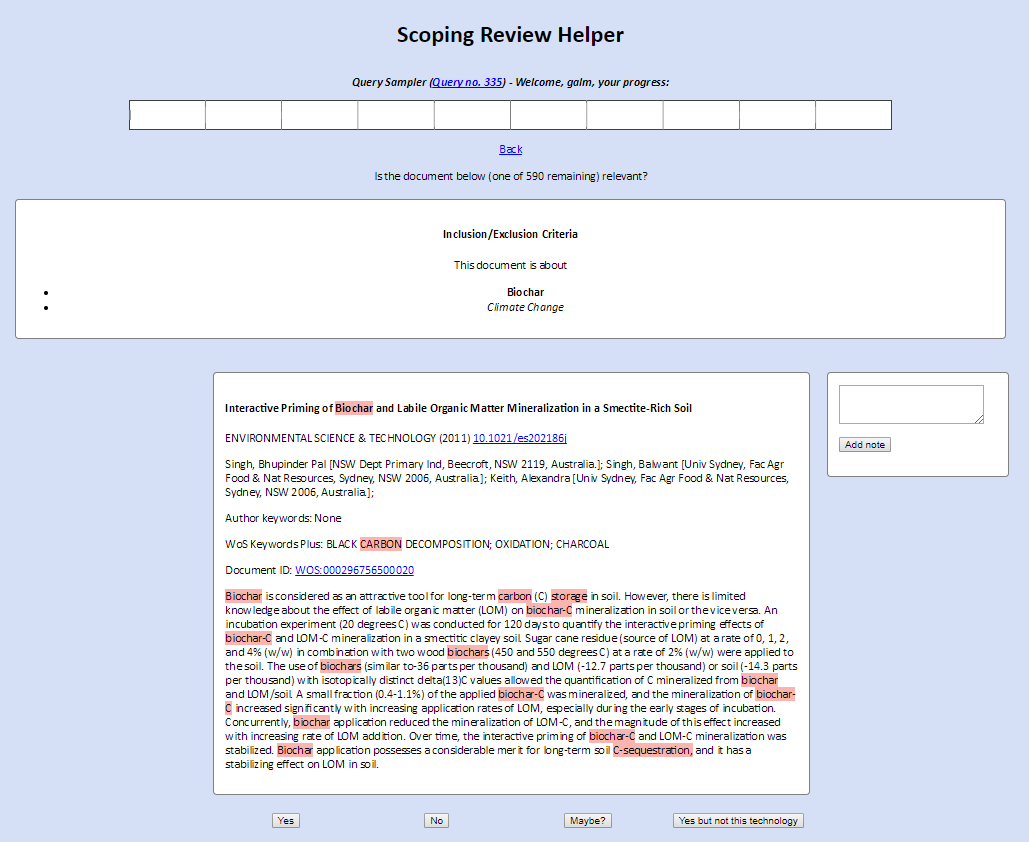
\includegraphics[width=0.85\linewidth]{images/screen.png}
			\end{figure}
			\begin{figure}
				\fbox{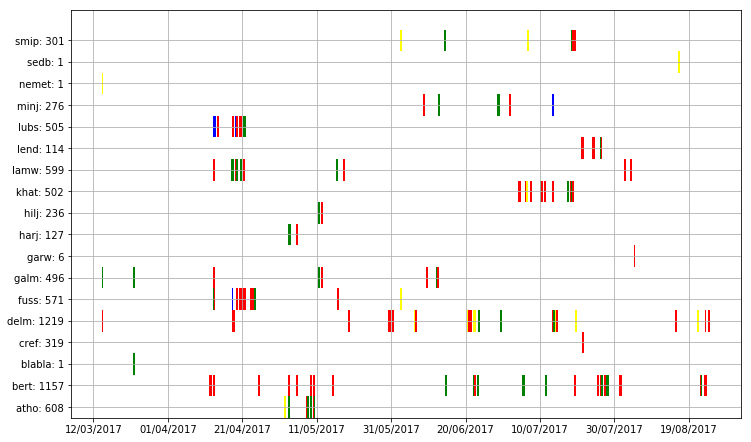
\includegraphics[width=0.85\linewidth]{images/ratings_user_time.png}}
			\end{figure}
		\end{center}
	\end{column}
	\begin{column}{0.5\linewidth}
		\begin{center}
			\begin{itemize}
				\item A tool for teams to manage documents downloaded from online databases
				\item Teams can screen documents and mark them as relevant or not
			\end{itemize}
		\medskip
		\textbf{Extensions}
		\begin{itemize}
			\item Snowballing (getting more documents by looking through references and citations)
			\item Automatically emailing authors in the database and asking them to enter missing information
		\end{itemize}
		\end{center}
	\end{column}
\end{columns}

\end{frame}

\begin{frame}{Scientometric Analysis}

\begin{columns}
	\begin{column}{0.5\linewidth}
		\begin{center}
			\begin{figure}
				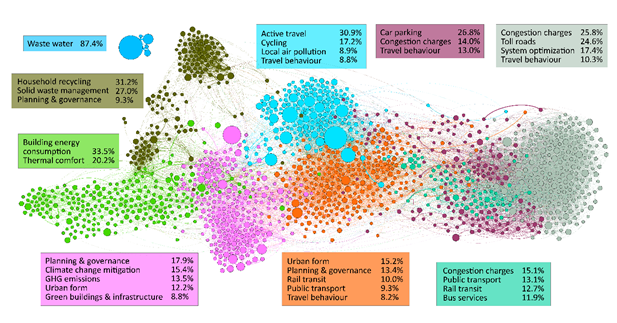
\includegraphics[width=1\linewidth]{images/network.png}
			\end{figure}
		\end{center}
	\end{column}
	\begin{column}{0.5\linewidth}
		\begin{center}
			Scientometric Analysis uses the reference information of articles to answer questions about an area of literature:
			\begin{itemize}
				\item What authors/institutions/articles play an important role?
				\item What is the community structure of a network of papers?
				\item How has an area of literature evolved? What are the roots of ideas, and how can we trace their development?
			\end{itemize}
		\end{center}
	\end{column}
\end{columns}

\end{frame}

\begin{frame}{Topic modelling}

\begin{columns}
	\begin{column}{0.5\linewidth}
		\begin{center}
			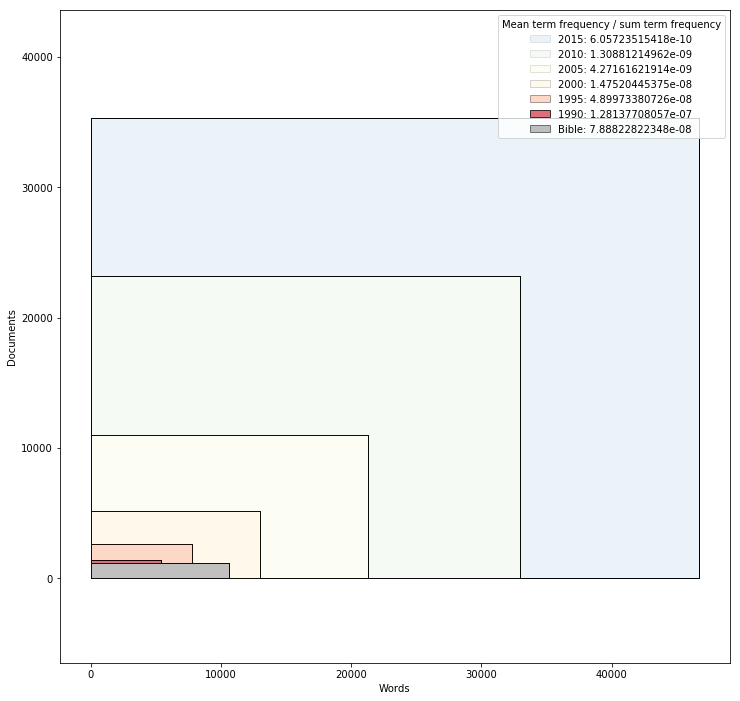
\includegraphics[width=\linewidth]{images/volume_variety_bible.png}
		\end{center}
	\end{column}
	\begin{column}{0.5\linewidth}
		\begin{center}
			\begin{itemize}
				\item Topic modelling is a way of reducing the dimensionality of a corpus of documents
				\item A large matrix of documents x words is factorised by
				a matrix of topics x words and a matrix of topics x documents
				\citep{Lee1999}
				\item Topics describe the latent structure of the document corpus
				\item There are a number of different models, with different assumptions, and different approaches to estimation. A very good introduction to the concept is found in \citet{Blei2012}
			\end{itemize}
		\end{center}
	\end{column}
\end{columns}

\end{frame}

\begin{frame}{Topic modelling}

\begin{columns}
	\begin{column}{0.5\linewidth}
		\begin{center}
	\fbox{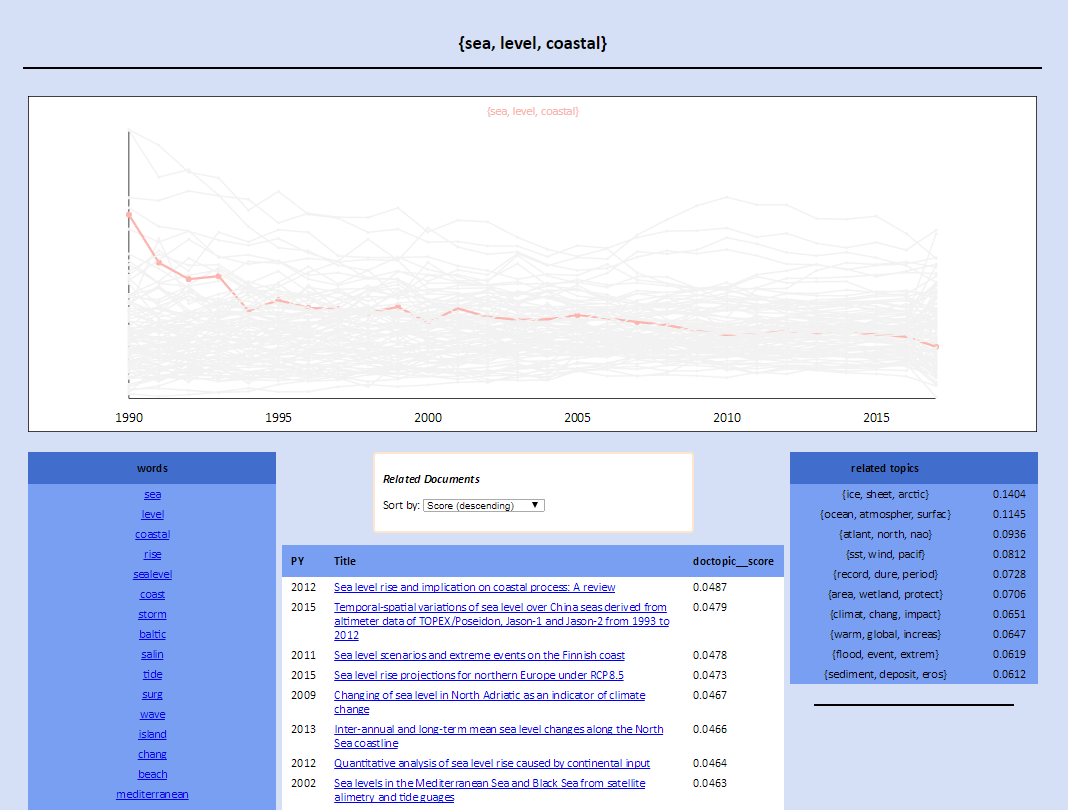
\includegraphics[width=0.95\linewidth]{images/topic.png}}
\end{center}
	\end{column}
	\begin{column}{0.5\linewidth}
		\begin{center}
			\fbox{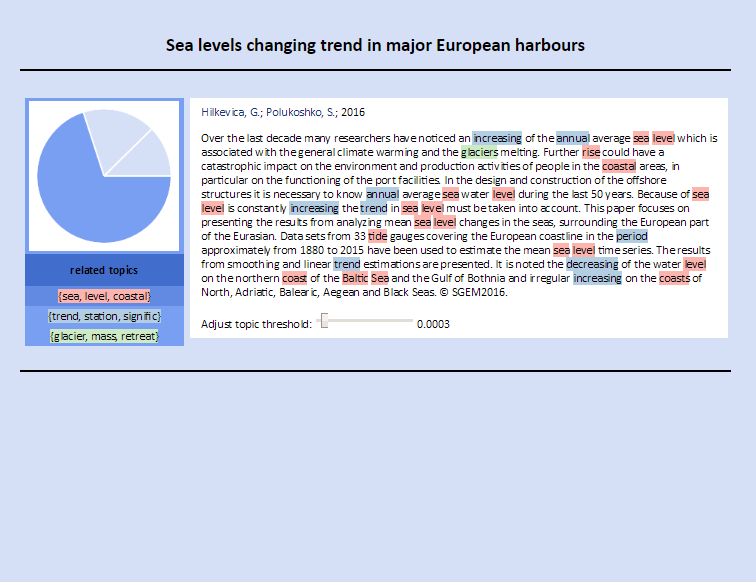
\includegraphics[width=0.95\linewidth]{images/document.png}}
		\end{center}
	\end{column}
\end{columns}

\end{frame}



\begin{frame}{Topic modelling}

\begin{columns}
	\begin{column}{0.4\linewidth}
		\begin{center}
			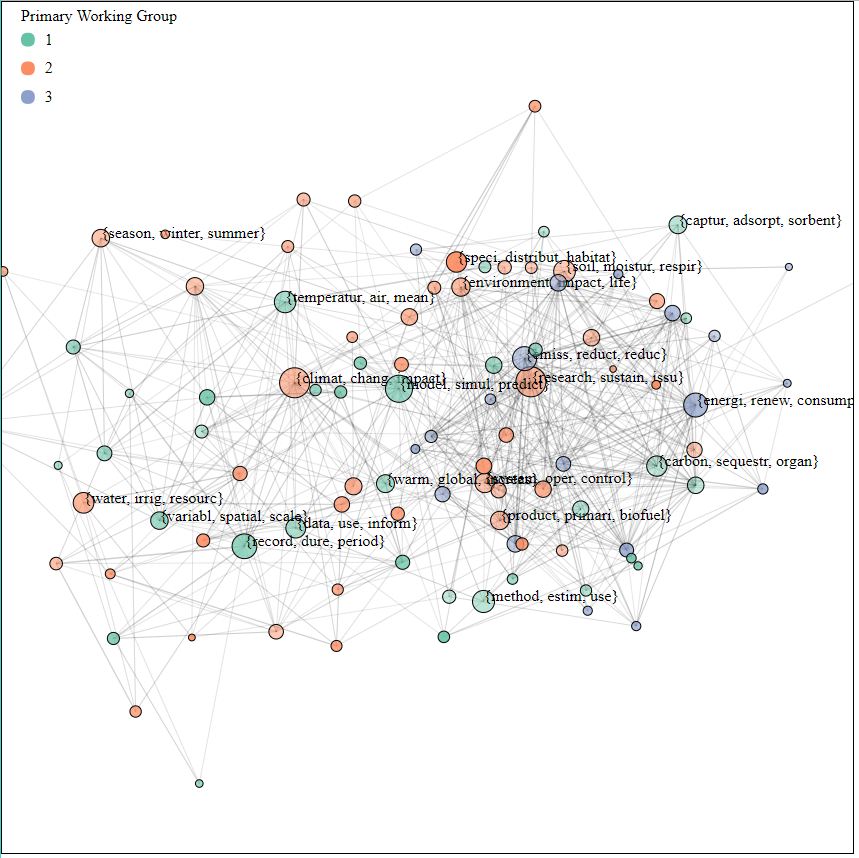
\includegraphics[width=1\linewidth]{images/network_wg_65.png}

			
		\end{center}
	\end{column}
	\begin{column}{0.6\linewidth}
		\begin{center}
			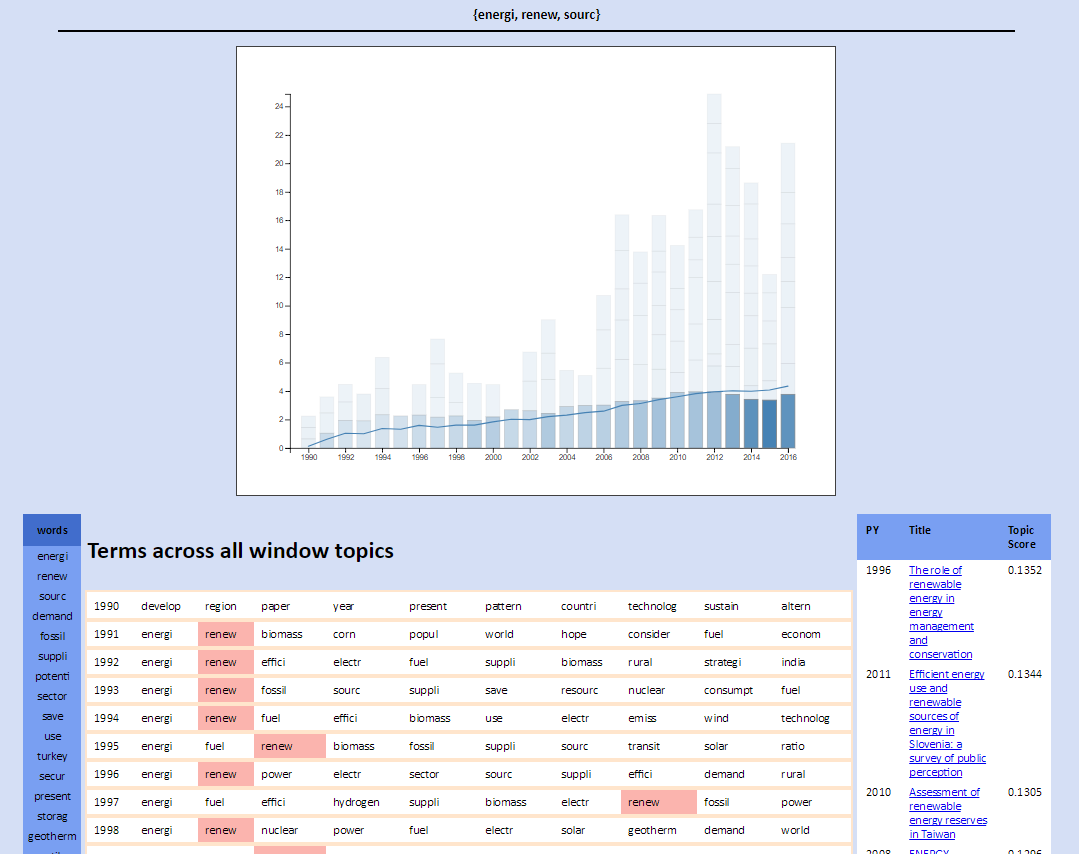
\includegraphics[width=0.7\linewidth]{images/time_renewed.png}
			\begin{itemize}
				\item How do topics relate to one another?
				\item How do topics change over time? \citep{Greene2016}
				\item How can we incorporate other information into the topic model? \citep{Tvinnereim2015, Roberts2014a}
				\item Topic models of speech \citep{El-Assady2016}
				
			\end{itemize}
		\end{center}
	\end{column}
\end{columns}

\end{frame}




\begin{frame}{Other Text Analysis}

\begin{columns}
	\begin{column}{0.5\linewidth}
		\begin{center}
			\fbox{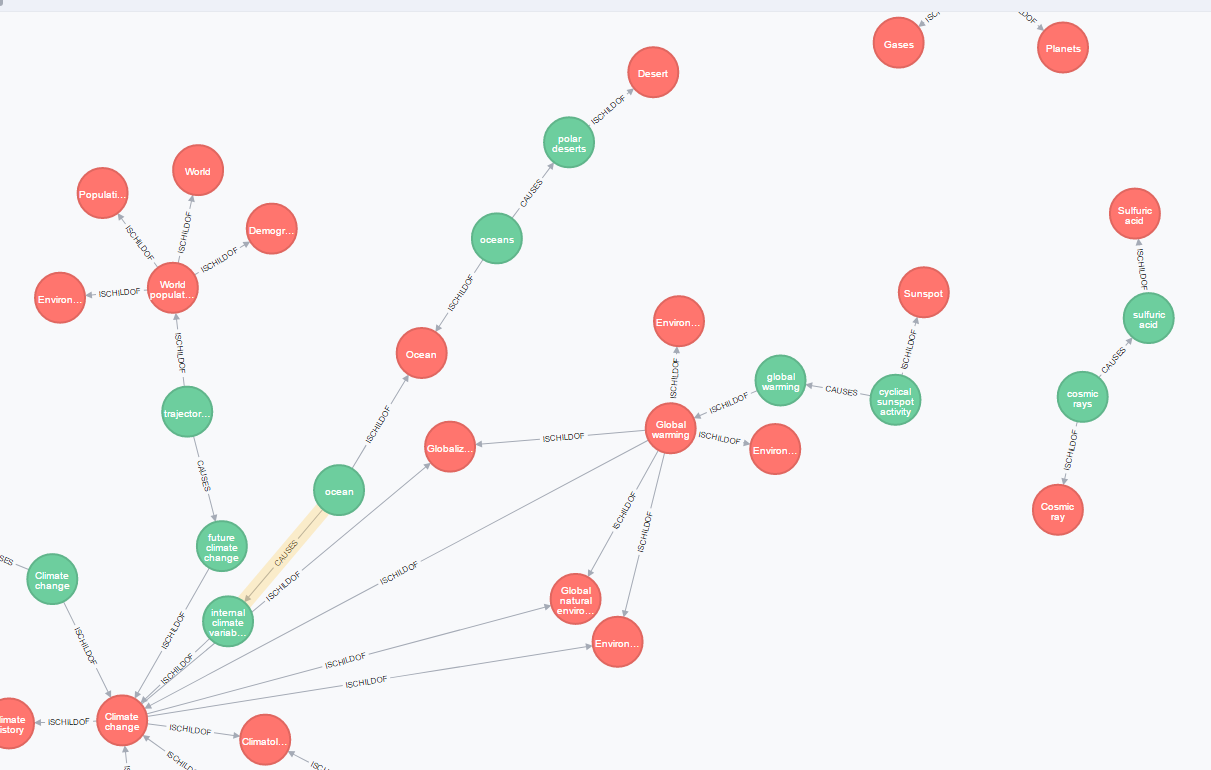
\includegraphics[width=\linewidth]{images/extract_raw.png}}
		\end{center}
	\end{column}
	\begin{column}{0.5\linewidth}
		\begin{center}
			\begin{itemize}
				\item Causaly collect causal statements from literature
				\item They aim to quantify and aggregate the strength of claims
				
			\end{itemize}
		\medskip
		\textbf{Applications?}
		\begin{itemize}
			\item Do we get more consolidated knowledge about causal relationships over time (in some WGs over others)?
			\item What can we learn about co-benefits and side-effects of different negative emission technologies?
		
				
			\end{itemize}
		\end{center}
	\end{column}
\end{columns}

\end{frame}



\begin{frame}{Frame Title}
	\small
	%\bibliography{/home/max/Documents/library/bibliography}
	\bibliography{C:/Users/galm/Documents/library/library}
\end{frame}

\end{document}
